
\chapter{Introduction} \label{ch:introduction}


%\begin{document}
%	\begin{figure}%
%		\centering
%		\subfloat[label 1]{{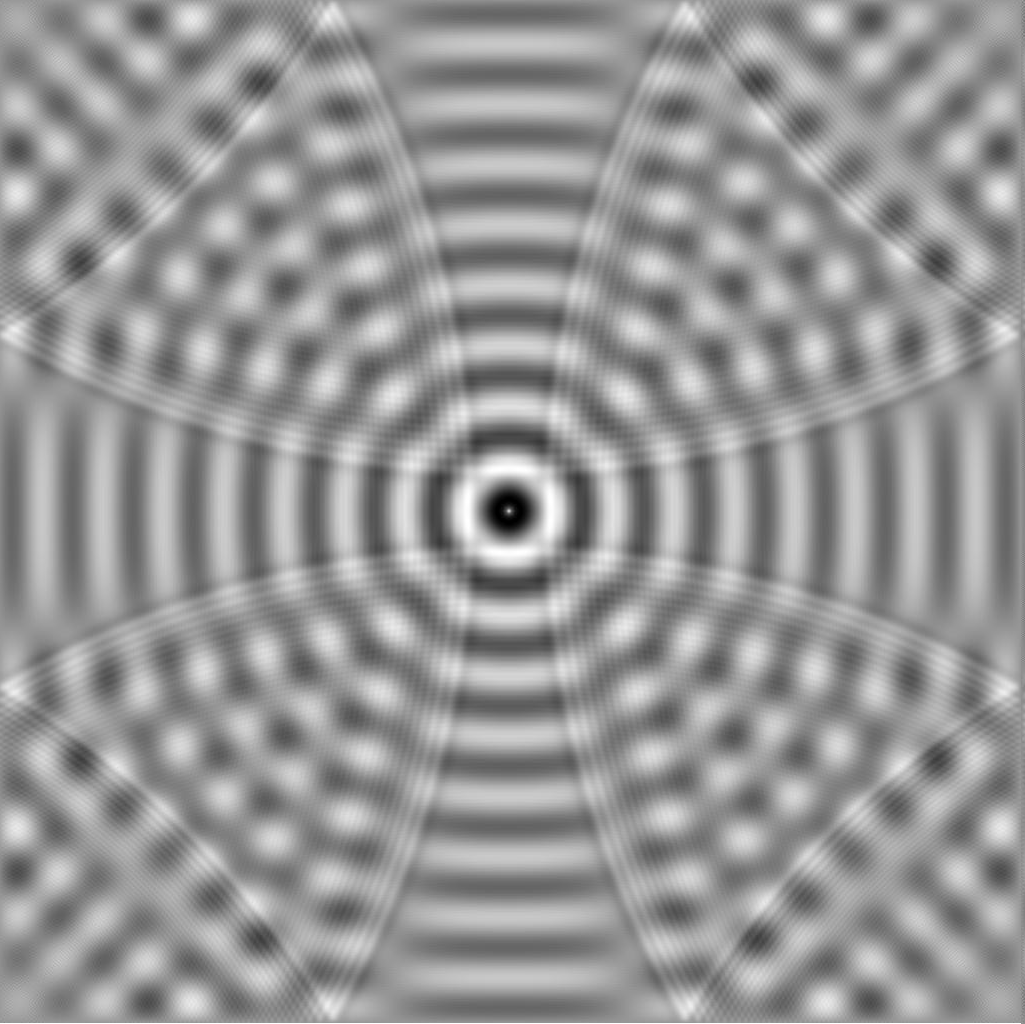
\includegraphics[width=5cm]{point-source-comparison-golightly.png} }}%
%		\qquad
%		\subfloat[label 2]{{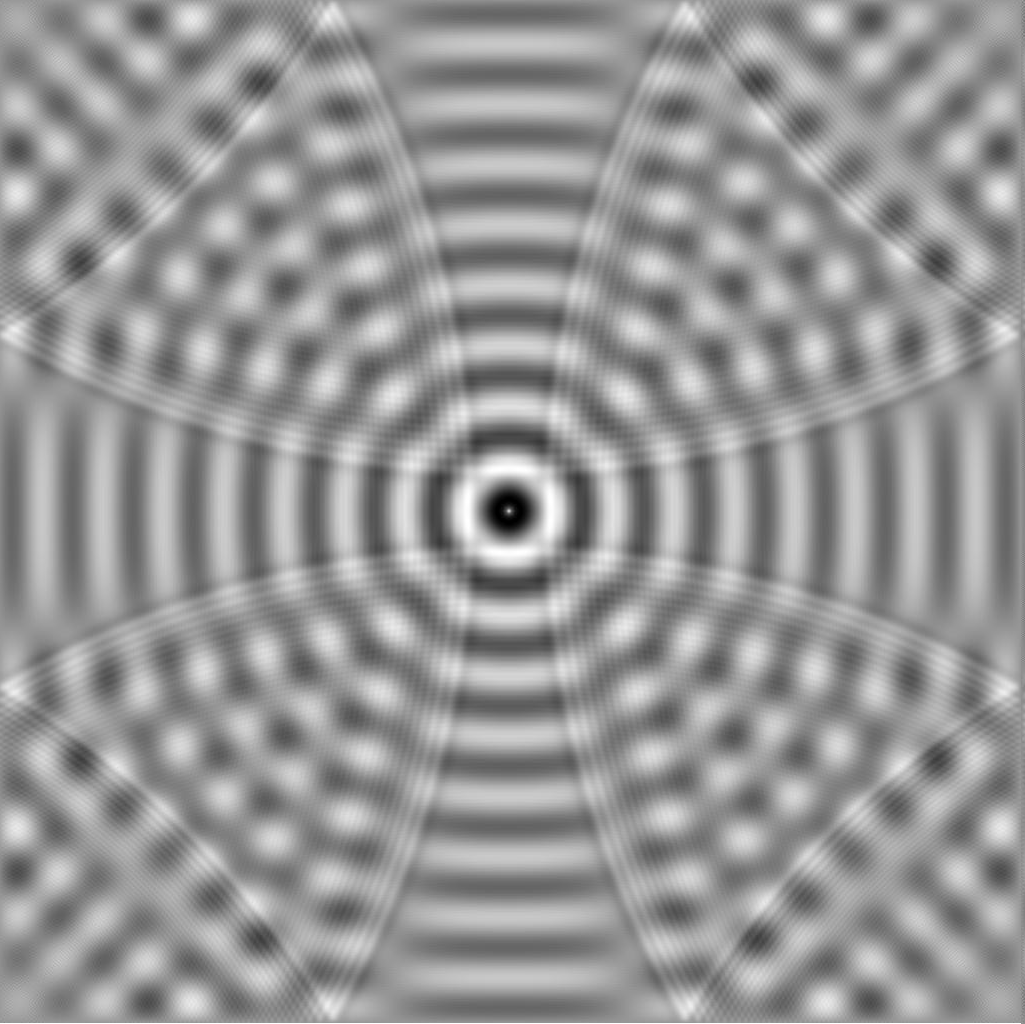
\includegraphics[width=5cm]{point-source-comparison-golightly.png} }}%
%		\caption{2 Figures side by side}%
%		\label{fig:example}%
%	\end{figure}
%\end{document}

%\begin{figure}[H]
%	\centering
%	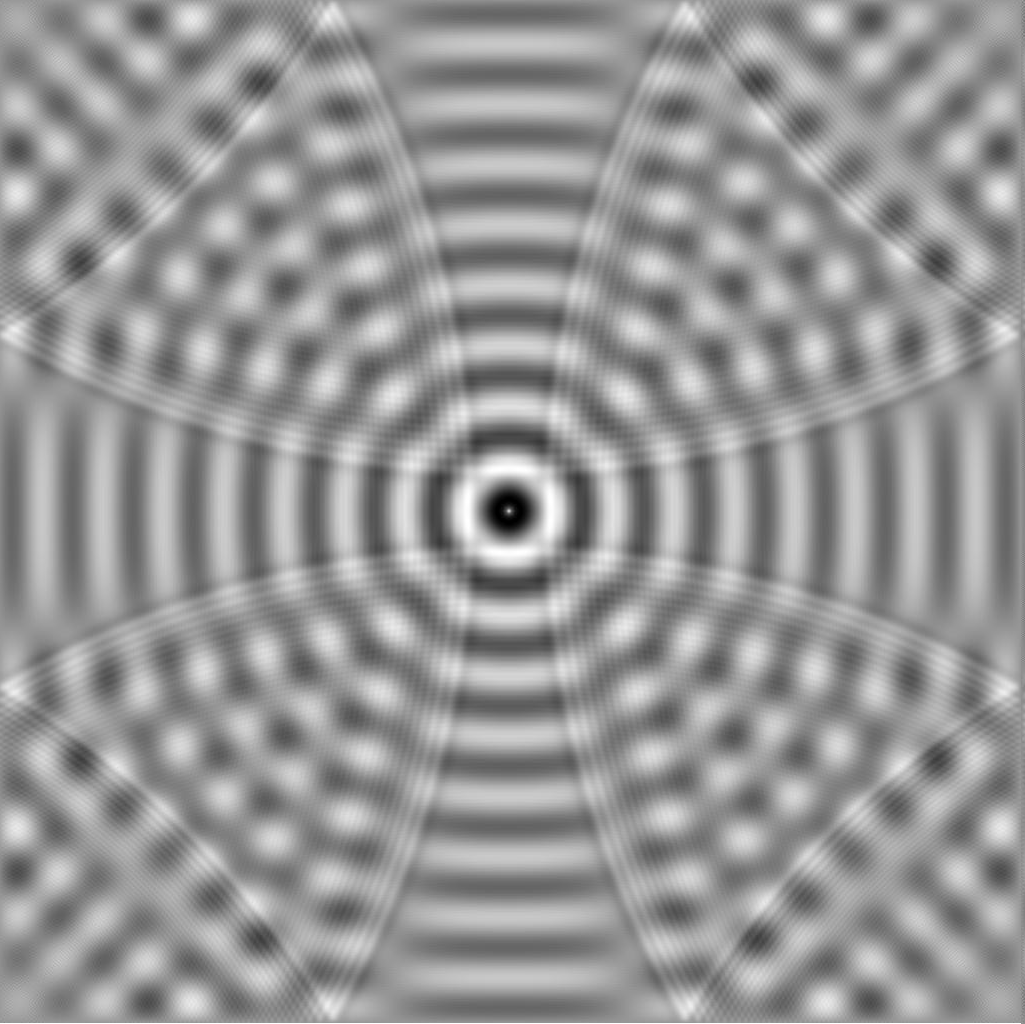
\includegraphics[width=\textwidth,
%	keepaspectratio]{point-source-comparison-golightly.png}
%	\caption{GoLightly (left) and Meep (right). $TM_Z$ $E_Z$ result for a point source with Dirlecht boundary.}
%	\label{fig:pointSourceComparison}
%\end{figure}


The Finite Difference Time Domain (FDTD)\cite{Yee} method is an electromagnetic wave simulation algorithm employed by many commercial simulation and design packages, as well as open source software such as MIT's Meep\cite{OskooiRo10}. 

Given the computationally-intensive nature of FDTD, organizations requiring simulation of large domains or complex circuits must provide significant resources. These may take the form of leased server time or utilization of an on-site high-performance cluster, amongst other options.

In this thesis, we explore an implementation of FDTD utilizing graphics processing units (GPUs) via NVIDIA's CUDA\cite{cuda} language. Initially designed to perform image generation tasks such as those required by games, cinema and related fields, modern versions are well-suited for general computation work. GPUs are now enjoying wide adoption in fields such as machine learning\cite{Raina09largescaledeep} and artificial intelligence\cite{wu2009clustering}, medical research\cite{QIMS1079} and other areas which require rapid analysis of large datasets.

Multi-core CPUs excel at quickly performing disparate operations on potentially-unrelated data. This is a requirement in traditional desktop computing. However, the flexible architecture that provides this capability can be a liability when repeatedly executing large batches of identical operations. 

GPUs trade this flexibility for increased throughput. Modern consumer-grade GPUs offer thousands or tens of thousands of processing units ("cores"). Some algorithms, such as FDTD, require little or no data interdependence, no branching logic (a severe performance impediment on GPUs) and consist of short cycles of simple operations. The power of the GPU lies in performing these simple operations at large scale, with thousands of threads running in parallel. 

The following sections detail the FDTD algorithm. Later sections describe a CPU-based implementation (MIT's  Meep), and our GPU-based GoLightly simulator. We verify the GPU solution numerically, and compare performance between CPU- and GPU-based implementations. Finally, we consider future applications and enhancements. 

